\chapter{The ATLAS Trigger System}
\label{sec:trig}

In 2015 and 2016, the LHC has been colliding proton beams with a beam bunch spacing of \SI{25}{\nano\second},
meaning that the ATLAS experiment has been taking data at a rate of 40 MHz.
Due to the large computing resources required to process and store each event,
it is not possible to record all events.
The most interesting events to study contain a hard-scatter collision,
defined as collisions in which the momentum transfer is large compared to the proton mass~\cite{trig-hard_scatter},
as these are the collisions that, for example, can produce a TeV scale BSM particle.
Therefore, the ATLAS experiment uses a trigger system to select events that contain
contain a high-$p_{T}$ physics object which indicates that a hard-scatter collision has occured.

The ATLAS trigger-system consists of two levels;
the first level trigger (L1) and the higher level trigger (HLT) \cite{det-run2_trigger}.
Figure~\ref{fig:det-trigger_schem} shows a schematic outlining the trigger system used in Run-2 \cite{det-run2_triggerPerf}. 

The L1 trigger is hardware based and reduces the rate from 40~MHz to 100~kHz within a time window of \SI{2.2}{\micro\second}.
The L1 trigger uses custom electronics to rapidly process information directly from the
calorimeter and Muon Spectrometer, searching for high-$p_{T}$ muon tracks and large energy depositys in the calorimeter.
The central trigger processor then uses a set of pre-defined conditions
to decide if a L1 trigger accept is given and thus events are passed on to the next step of triggering.
At the same time Regions of Interests (ROIs) are constructed around the high-\pT{} objects indentified by the L1 trigger, which are passed on to the HLT. 

The next step is the HLT, a software based trigger,
which further reduces the event rate to 1~kHz within a time window of ~\SI{0.2}{\second}.
The HLT uses the information from the full detector
to perform a more complete reconstruction of the physics objects within the event,
the most time consuming reconstruction algorithms only being run only within the ROIs taken from L1.
The more complex event analysis within the software-based trigger includes
track reconstruction and therefore allows for $b$-jet identification.
If the content of the event reconstruction passes a pre-set criteria, a HLT accept is issued
meaning that the events are passed on for processing and storage. 
% in offline computer farms (known as tier-0).

\begin{figure}[!htb]
  \begin{center}
    \includegraphics[width=1\linewidth, angle=0]{figs/Detector/trigger_schem.png}
  \end{center}
  \caption[A schematic of the ATLAS trigger and data-acquisition system in Run-2, with a focus on the components required for triggering.]
          {A schematic of the ATLAS trigger and data-acquisition system in Run-2, with a focus on the components required for triggering~\cite{det-run2_trigger}.}
  \label{fig:det-trigger_schem}
\end{figure}

In the ATLAS trigger system there is an additional process known as pre-scaling that can be applied.
If a trigger is pre-scaled, only a fraction of the events that pass the trigger are recorded.
Pre-scaling is applied to maintain the output rate of the L1 and HLT trigger systems at 100 and 1~kHz respectively as the instantanous luminosity of the LHC collisions is increased.
An unprescaled trigger is defined as a trigger that has no prescale applied to it.
Most analyses at ATLAS use unprescaled triggers to maximise the acceptance of the trigger.

%In the di-$b$-jet searches presented in this thesis, two different trigger strategies are used.
%A single jet trigger is used for the high-mass di-$b$-jet search and a double $b$-jet trigger for the low-mass di-$b$-jet search.
This chapter describes triggers used in the two di-$b$-jet searches presented in this thesis in Chatper~\ref{sec:evt}~-~\ref{sec:lim}.
Section~\ref{sec:trig-jet} describes jet triggers that are used in the high-mass di-$b$-jet search,
Section~\ref{sec:trig-bjet} describes $b$-jet triggers that are used in the low-mass di-$b$-jet search
and finally Section~\ref{sec:trig-bjet_eff} presents the measurement of the $b$-jet trigger efficiency, an essential input of the low-mass search.

There are two important definitions used in this chapter, and throughout this thesis.
\textit{`Online'} refers to any algorithms run or objects reconstructed at the trigger level.
\textit{`Offline'} refers to algorithms run after events have passed the trigger at the data-processing level.
Offline algorithms and objects used in this thesis are described in Chapter~\ref{sec:obj}.

\section{Jet Triggers}
\label{sec:trig-jet}

Section~\ref{sec:obj-jets} described that hadronic jets are built from energy deposits in the ATLAS calorimeter.
Jet triggers are tasked with selecting events that contain with one or more high-\pT{} jets,
which is challenging at hadron colliders due to the extremely high cross-sections of hadronic jet production~\cite{trig-run2_proc}.
In Run-2 the jet triggers are used at both the L1 and HLT level, which are described at the begining of this section.

%\subsection{Level 1}

%The L1 trigger is a hardware based trigger which accepts or rejects an event within \SI{2.2}{\micro\second}.
The L1 jet trigger uses trigger towers which are defined as energy deposits in a region of 0.1 x 0.1 in the $\eta-\phi$ plane integrated radially over all layers of the EM and hadronic calorimeter.
The L1 jet trigger accepts an event if a neighbouring group of 4x4 trigger towers containing energy deposits above some pre-set threshold is found.
The di-$b$-jet searches use the L1 trigger known as \verb|L1_J100|, which requires that at least one trigger tower group with an energy deposit of \SI{100}{\GeV} has been found.
Coarser jet reconstruction techniques relative to offline are used by the L1 trigger to be able to make a trigger decision within \SI{2.2}{\micro\second}.
%Other L1 triggers that search for multiple clusters are also possible to reduce the energy thresholds required.
%The L1 trigger then seeds the HLT trigger.
In the  L1 trigger there is no tracking information, meaning that electron and taus
are also triggered on using similar techniques as hadronic jet algorithms, except using narrower groups of trigger towers.

%\subsection{HLT}

The HLT jet trigger, due to larger time allowed for a trigger decision,
is able to use more complex algorithms to reconstruct jets.
At the HLT level jets are reconstructed using hadronic topoclusters formed from EM or hadronic calorimeter cells and the anti-$k_T$ jet-reconstruction algorithm with $R$=0.4;
topoclusters and the anti-$k_T$ algorithms are described in Section~\ref{sec:obj-jets}.
The HLT jet trigger is passed if the reconstructed jets pass a pre-set criteria that depends on the number and $p_T$ of the jets.

%\subsection{High-mass trigger selection}

For the high-mass di-$b$-jet search the \verb|HLT_j380| trigger is used, which requires that at least one jet is found with a $p_T >$ 380 GeV.
This is chosen as it is the unprescaled single jet trigger with the lowest cut on jet-$\pT$ in 2016 data-taking.
%meaning that of triggers that accept every event passing a single jet criteria,
%this trigger has the lowest jet-$p_T$ threshold.
%Due to the exponential increase in jet production cross-section at low jet-$p_T$,
%the $p_T$ threshold is set to keep the acceptance rates low enough such that the HLT trigger is within its output rate budget of 1~kHz.

However, as will be shown in Section~\ref{sec:evt},
the online jet $p_T$ threshold limits the mass region that the high-mass di-$b$-jet can probe to $m > 1.1$~TeV.
In the mass region $m < 1.1$~TeV a kinematic bias from the online jet $p_T$ threshold is introduced
such that the backgrounds from the Standard Model cannot be modelled. 
Therefore, for a di-$b$-jet search to probe lower masses a different trigger strategy is required.

\section{$b$-Jet Triggers}
\label{sec:trig-bjet}

As described in Section~\ref{sec:obj-bjets}, $b$-jets, defined as jets containing a $b$-hadron,
can be identified from the topology of tracks in a process known as $b$-tagging.
$b$-Tagging can be utilised online to reduce rates of jets significantly~\footnote{\ As described in Section~\ref{sec:theo-qcd-dijet_features},
  the QCD dijet production is dominated by light-jets}
allowing for a lower jet-$p_T$ threshold than is used by the single jet-$p_T$ trigger.
Hence, using a $b$-jet trigger in di-$b$-jet searches means that a lower mass range can be probed.
%$b$-Jet triggers have been used previous ATLAS analyses,
%for example searches for exotic particles decaying to 4 $b$-jets via a pair of Higgs bosons~\cite{trig-H4b}.

The $b$-jet trigger utilises the regions of interest (RoI) defined by the jets reconstructed in the L1 jet trigger.
The $b$-jet trigger procedure for 2016 data-taking contains three steps~\cite{trig-bTrig_desc}.
Firstly, a `fast'-tracking algorithm is run in a super-RoI,
which is a superset of all RoIs which corrspond to a L1 jet with $\pT{} >$ 30 GeV.
The reconstructed tracks are then used to identify the hard-scatter primary vertex (PV) in the event.
Secondly, within each jet RoI precision tracking is run, with a constraint on the PV position from the first step.
Finally, these tracks are the input to the MV2 $b$-tagging algorithm, described in Section~\ref{sec:obj-bjets_MV2}, used to identify $b$-jets.

Figure~\ref{fig:trig-bTrig_perf} shows the $b$-jet efficiency against light-jet and $c$-jet rejection
of online $b$-tagging for a variety of $b$-jet trigger configurations in simulated $t\bar{t}$ events.
The black line represents MV2c20 algorithm used in 2016 data-taking is described in Section~\ref{sec:obj-bjets_MV2}.
The blue line represents the IP3D+SV1 algorithm that combines two of the base $b$-tagging algorithms, described in Section~\ref{sec:obj-bjets}.
IP3D+SV1 was used by the $b$-jet trigger in 2015 data-taking.

\begin{figure}[!ht]
  \begin{center}
    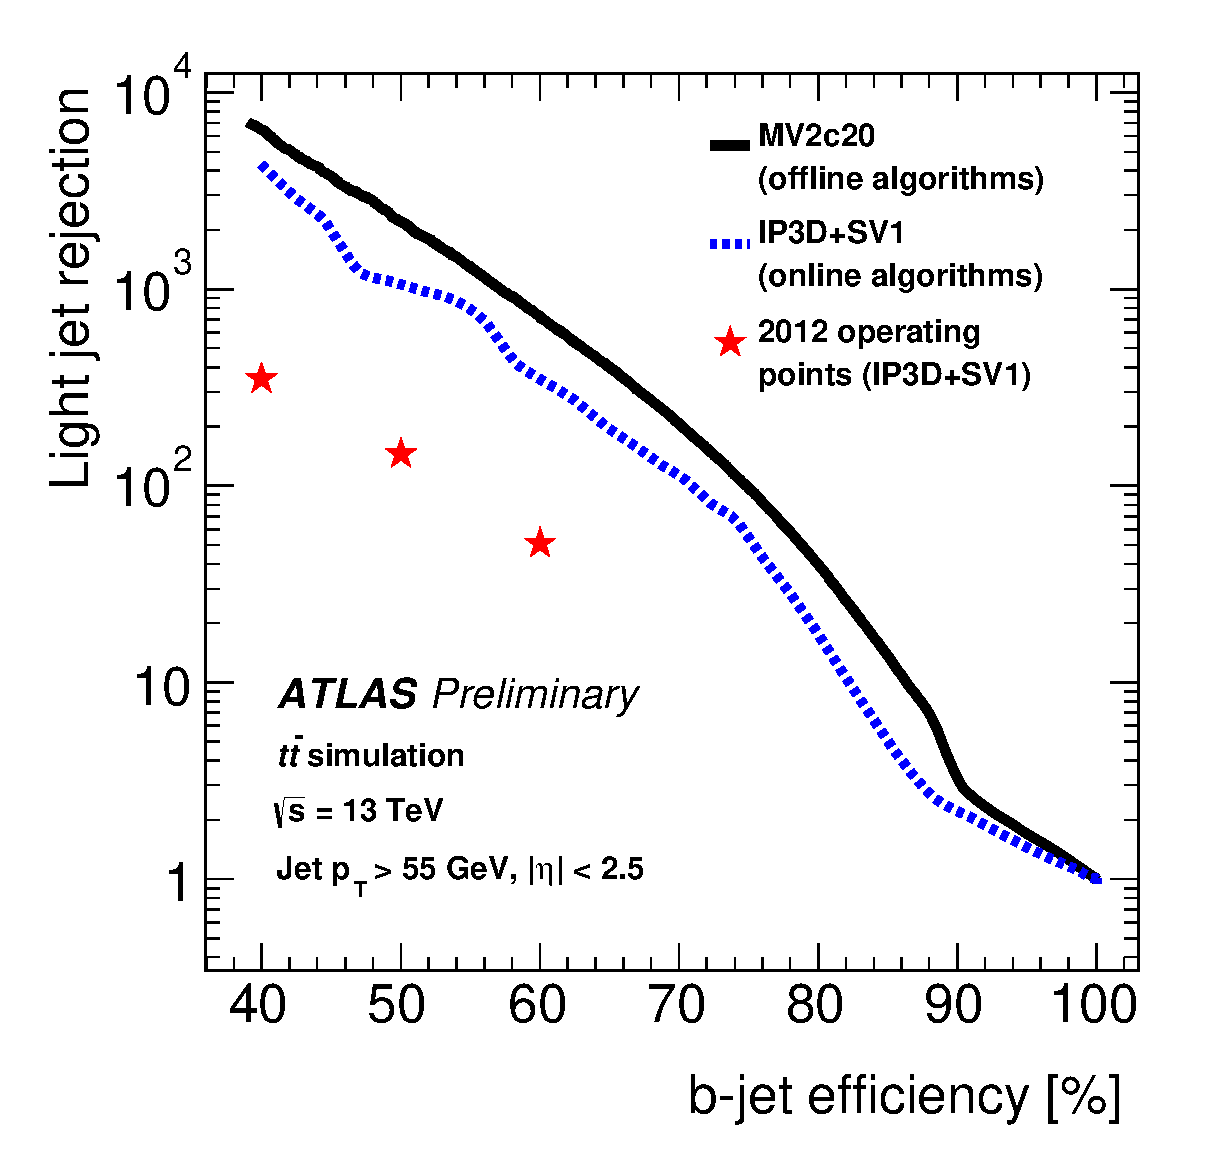
\includegraphics[width=0.48\linewidth, angle=0]{figs/Trigger/trig-bTrig_perf_light.eps}
    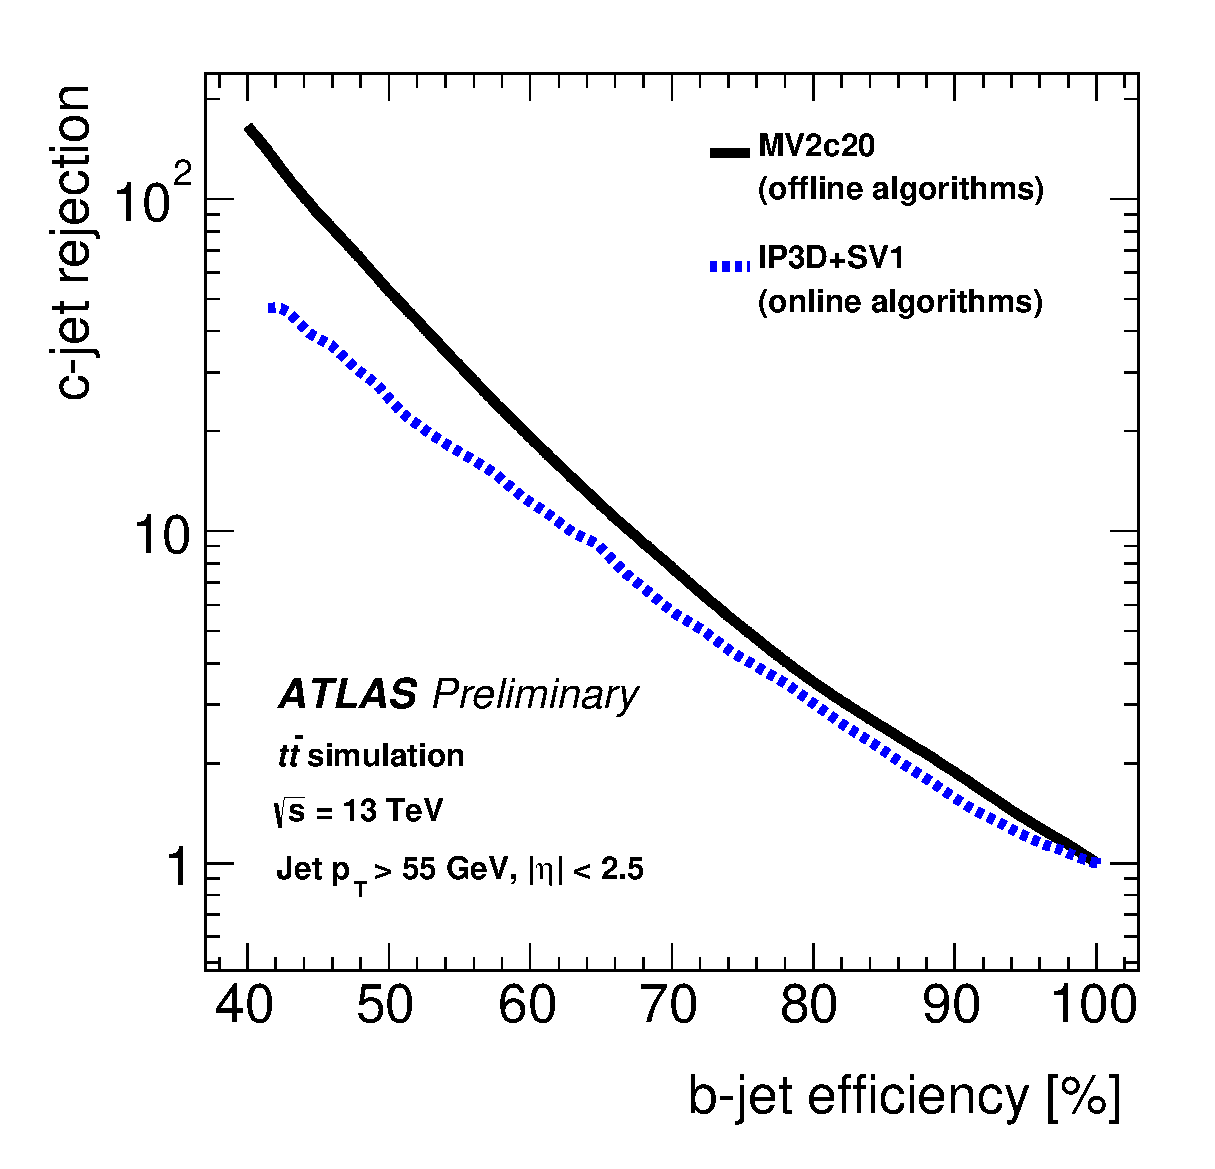
\includegraphics[width=0.48\linewidth, angle=0]{figs/Trigger/trig-bTrig_perf_charm.eps}
  \end{center}
  \caption[The expected $b$-jet efficiency of $b$-jet triggers in Run-2 compared to the set-up used in 2012 data-taking.]
    {The expected $b$-jet efficiency of $b$-jet triggers with respect to (a) light-jet and (b) $c$-jet rejection
    in the case where the $b$-tagging algorithm used is MV2c20 (black), IP3D+SV1 (blue) and for the set-up used in 2012 data-taking (red stars)~\cite{trig-bTrig_desc}.}
  \label{fig:trig-bTrig_perf}
\end{figure}

\newpage
There are several $b$-jet triggers avaliable;
with a variety of requirements on the jet multiplicity, number of tagged jets and $b$-tag operating point used.
As the signal considered in the low mass di-$b$-jet search is a BSM particle decaying to two $b$-quarks, a double $b$-jet trigger is used.
The double $b$-jet trigger requires that there are two jets with $p_T >$ 150 and 50 GeV respectively,
which have been $b$-tagged at the 60\% efficiency operating point \footnote{The trigger is known as \textit{HLT\_j150\_bmv2c2060\_split\_j50\_bmv2c2060\_split}.}.
It will be shown in Chapter~\ref{sec:evt} that the low mass di-$b$-jet search is able to probe the mass range $m >$ 0.57 TeV.

There are significant differences in the  $b$-jet trigger configurations used in 2016 and 2015 data-taking.
Firstly, the $b$-tagging algorithm is MV2c20 in 2016 data-taking whilst IP3D+SV1 was used in 2015 data-taking.
MV2c20 is used in 2016 due to improved $b$-tagging performance, as shown in Figure~\ref{fig:trig-bTrig_perf}.
Secondly, different algorithms were used to identify the hard-scatter primary vertex in 2015 and 2016 data.
2016 data-taking employs the \verb|xPrmVtx| algorithm, which is based on the hard-scatter primary vertex finding algorihm used offline, as described in Section~\ref{sec:obj-tracks_pv}.
In 2015 data-taking the \verb|EFHist| algorithm is employed, which uses a simple histogram based approach to identify the hard-scatter primary vertex.
As a result of these significant differences, data taken in 2015 and 2016 by the $b$-jet trigger are not easily combined in a di-$b$-jet search.
Therefore, as described in Chapter~\ref{sec:evt}, the low mass di-$b$-jet search uses the 2016 data-set which has a significantly larger instantaneous luminosity.

In addition there are important differences between online and offline $b$-tagging.
Firstly, coarser tracking information is available online, notably online tracks are not reconstructed from the whole range of the detector due to the large time required to reconstruct tracks.
Secondly, Section~\ref{sec:obj-bjets_MV2} a simulated sample containing $b$, $c$ and light-jets is used to train the MV2 algorithm.
A different fraction of $c$-jets were present in the training sample used to train the MV2 algorithm in online and offline $b$-tagging;
specifically 10\% were used offline (MV2c10) and 20\% were used online (MV2c20).
The reason MV2c20 is used online in 2016 data-taking is that the $b$-jet trigger configuration
had to be determined before the start of data-taking in March 2016,
whilst the reccomendation to use MV2c10 was announced internally in May 2016.
As offline and online $b$-tagging are significantly different, online $b$-tagging must have an independant calibration, which is described in the following section.

\newpage
\section{Efficiency Measurement of the $b$-Jet Trigger}
\label{sec:trig-bjet_eff}

The trigger strategy used by an analysis can have a large impact on the result,
therefore the trigger performance must be understood and calibrated.
This section desribes the \mbox{$b$-jet} trigger efficiency measurement in 2016 data-taking,
which is an important input to the low-mass di-$b$-jet search.

\subsection{Strategy}
\label{sec:trig-bjet_strat}

The $b$-jet trigger is always used in tandem with offline $b$-tagging which is calibrated independently of the $b$-trigger.
%As mentioned before, there are many differences between offline and online $b$-tagging.
Therefore, the $b$-jet trigger efficiency, $\epsilon_{b\text{Trig}}$, is defined with respect to offline $b$-tagging:
Specifically, $\epsilon_{b\text{Trig}}$ is defined as the number of $b$-jets that are offline $b$-tagged and match an online $b$-tagged trigger-jet
divided by the number of $b$-jets that are offline $b$-tagged and match a trigger jet.
Or to put this in an equation;
\begin{equation}
 \epsilon_{b\text{Trig}} = \frac{N(\text{Offline-tagged, online-tagged, $b$-jets)}}{N(\text{Offline-tagged, trigger-matched, $b$-jets)}}
\end{equation}
The process used to match trigger jets and offline jets is described in Section~\ref{sec:trig-evtSel}.
%$\epsilon_{b\text{Trig}}$ is probability if a $b$-jet is produced in a proton collitions,
%the jet will be $b$-tagged at the online level given that it created jet at the trigger level and that it would be $b$-tagged offline.

As is done for offline $b$-tagging, as described in Section~\ref{sec:obj-bjets_calib},
the $b$-jet trigger efficiency is measured in both data and Monte-Carlo simulated samples.
Then a $b$-jet trigger data/MC scale factor for the  ($SF_{\,b\text{Trig}}$), is derived, where:
\begin{equation}
 SF_{\,b\text{Trig}} = \epsilon_{\,b\text{Trig}}^{\text{Data}}/\epsilon_{\,b\text{Trig}}^{\text{MC}}
\end{equation}
The data/MC scale-factor is applied to Monte-Carlo simulation when a $b$-jet trigger is used to correct for mismodelling of the $b$-jet trigger in simulation.
The data-sets, simulated samples and event selection used for the measurement of $b$-jet trigger efficiency are described below.

$b$-jet trigger efficiency and data/Monte-Carlo scale factors are derived for all combinations of offline and online $b$-tagging operating points.
However, only the process for the 70\% offline and 60\% online operating point are shown
as this is set of operating points used in the low mass di-$b$-jet seach;
details on the $b$-tagging operating points used are described in Chapter~\ref{evt}.

\newpage
\subsection{Description of Event Selection and Datasets}
\label{sec:trig-evtSel}

Di-lepton $t\bar{t}$ events containing a muon and an electron are selected to provide a high purity sample of $b$-jets to measure the $b$-jet trigger efficiency.
As discussed in Section~\ref{sec:theo-ttbar}, 
$e\mu$ di-lepton $t\bar{t}$ provides a distinctive signature to select events with and provides a pure sample $b$-jets required for the efficiency measurement.
Furthermore, the electron and muon provide a signature that can be used to select events at the trigger-level without using a $b$-jet trigger,
such that no bias is introduced from online $b$-tagging.

\noindent
Specifically, $e\mu$ di-lepton $t\bar{t}$ events are required to:
\begin{itemize}
\item Pass one of two single lepton $b$-performance triggers that require
    \begin{itemize}[label={$-$}]
    \item An online reconstructed medium muon with $\pT >$ 26 GeV.
    \item Or an online reconstructed electron with $\pT >$ 26 GeV \footnote{The triggers are called \textit{HLT\_mu26\_imedium\_2j35\_bperf} and \textit{HLT\_e26\_tight\_iloose\_2j35\_bperf} respectively.}.
    \end{itemize}
\item Contain $\geq$ 1 offline medium muon with $\pT>30~\GeV$ and no jet within $\Delta R$ of 0.4.
\item Contain $\geq$ 1 offline medium electron with $\pT>30~\GeV$.
\item Contain $\geq$ 2 offline $b$-tagged jets, defined as:
   \begin{itemize}[label={$-$}]
     \item Offline R=0.4 anti-$k_T$ jets.
     \item $\pT>35~\GeV$ and $|\eta|<2.5$.
     \item Offline $b$-tagged at the 85\%~operating point.
     \item The offline jet must be matched to an online jet.
    \end{itemize}
\end{itemize}

Details of muon, electron, jet and $b$-tagged jet object definition are in Chapter~\ref{sec:obj}.
%chapter ~\ref{sec:obj-lepton},~\ref{sec:obj-jets} and \ref{sec:obj-bjets}\textit{(sec:obj-bjet)} respectively.
Offline jets are matched to online jets if $\Delta R < 0.4$,
the matching is exclusive meaning that online jets are only matched to offline jets with the smallest $\Delta R$ seperation.

The triggers deployed are $b$-performance triggers, which are special triggers used in data-taking specifically for monitoring the $b$-jet trigger performance.
They required that an online muon or an electron with $\pT{} > 26$~\GeV~is reconstructed.
The $b$-performance triggers then run the online $b$-tagging algorithm on all trigger jets with $|\eta|<2.5$ and
$p_{T}>35$~\GeV~without performing any cuts on the output of the MV2c20 algorithm.
Therefore, $b$-performance triggers can select $e\mu$ di-lepton events at the trigger-level
and thus provide an unbiased source of online $b$-tagged jets to measure the $b$-jet trigger efficiency.

The data-set used is 13~TeV $pp$ collision data collected by the ATLAS detector between March and December 2016.
This is the same data-set used by the low mass di-$b$-jet search presented in this thesis, which is discussed in Chapter~\ref{sec:evt}.
A $b$-jet trigger aware Good Run List (GRL) 
\footnote{A GRL is effectively a list of lumi-blocks that pass certain data-quality requirements.
  A further discussion of GRLs are found in Section~\ref{sec:evt_datasets}.}
applies the requirement that the online beamspot $z$-position is within 2mm of the origin in Periods A-I of the data,
a discussion of the requirement for this GRL is in Section~\ref{sec:trig-grl}. 
After the application of the GRL the data-set corresponds to an integrated luminosity of 24.3~\ifb~of data.

A $e\mu$ di-lepton $t\bar{t}$ event selection with 2 $b$-tags
is dominated by $t\bar{t}$ events with a small contribution from single-top production~\cite{trig-ttbar};
the remaining backgrounds are negligible and are not considered in this efficiency measurement.
For the simulated sample; a Monte-Carlo simulated $t\bar{t}$ sample is produced using the
Powheg-Box v2~\cite{trig-powheg} generator with the CT10 PDF sets~\cite{trig-CT10} in the matrix element calculations.
For the simulated single-top sample electroweak t-channel, s-channel and $Wt$-channel single top-quark events are generated using the Powheg-Box v1 generator and CT10 PDF sets.
%This generator uses the 4-flavour scheme for the NLO matrix elements calculations together with the fixed four-flavour PDF
%For all top processes, top-quark spin correlations are preserved (for t-channel, top quarks are decayed using MadSpin[10a]).
For both processes the parton shower, fragmentation and the underlying event are simulated using Pythia6.428~\cite{trig-pythia6} with the CTEQ6L1~\cite{trig-CTEQ6L1} PDF sets
and the corresponding Perugia 2012 tune (P2012)~\cite{trig-perugia}.
The top mass is set to 172.5 GeV.
The EvtGen v1.2.0 program~\cite{trig-evtGen} is used to model the decays of $b$ and $c$ hadrons.

\subsection{Investigation of Data-Simulation Discrepancies}
\label{sec:trig-inv}

This section will present the observation and investigation of discrepanices between the $b$-jet trigger efficiency measured in 2016 data and simulation.
%and the investigation into the discrepancies.
%The results of the studies in this section will be used in Section~\ref{sec:trig-grl} to describe the solution that has been implamented. 
To replicate the event selection used during the discrepancy and investiation studies the $b$-jet trigger aware GRL is not applied in this section.
%Otherwise the event selection used is indentical to the event selection described in~\ref{sec:trig-evtSel}.
%except that no .%, the triggers %are single lepton triggers without the additional $b$-performance functionality
%\footnote{\ Specifically HLT\_mu26\_imedium and HLT\_e26\_tight\_iloose.}
%and the offline jets are not required to match a trigger jet to be included in the denominator of $b$-jet trigger efficiency calculation.
%Furthermore, for reasons of simplicity, only $t\bar{t}$ events are included in the simulated sample during the investigation studies.
%Hence, throughout this section simulation refers to $t\bar{t}$ events only.
%In Section~\ref{sec:trig-cross-checks} it will be shown that the effect of single-top production is small
%and would not affect the conclusions of the investigation studies.

Figure~\ref{fig:trig-Full_noGRL_eff_noHLTMatch} shows $b$-jet trigger efficiency against jet-\pT~and jet-$\eta$;
the efficiency in data is substantially below the efficiency expected from  simulation and has different distribution with respect to jet-$\eta$.
The substantial differences need to be investigated and understood. 

\begin{figure}[!t]
  \begin{center}
    \captionsetup[subfigure]{aboveskip=0pt,justification=centering}
    \subcaptionbox{Jet-\pT}{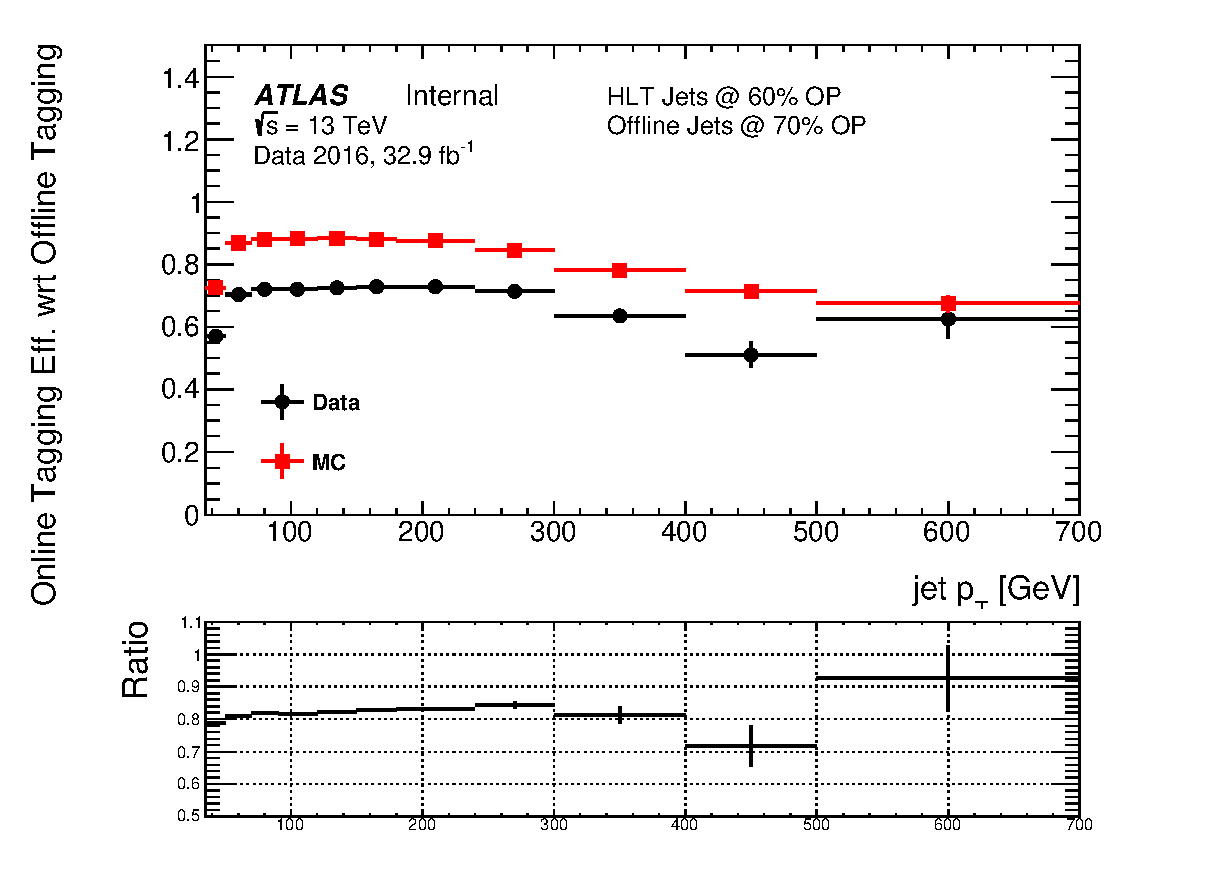
\includegraphics[width=0.48\linewidth, angle=0]{figs/trigger/Full_noGRL_eff_noHLTMatch_jetPt.eps} }
    \subcaptionbox{Jet-$\eta$}{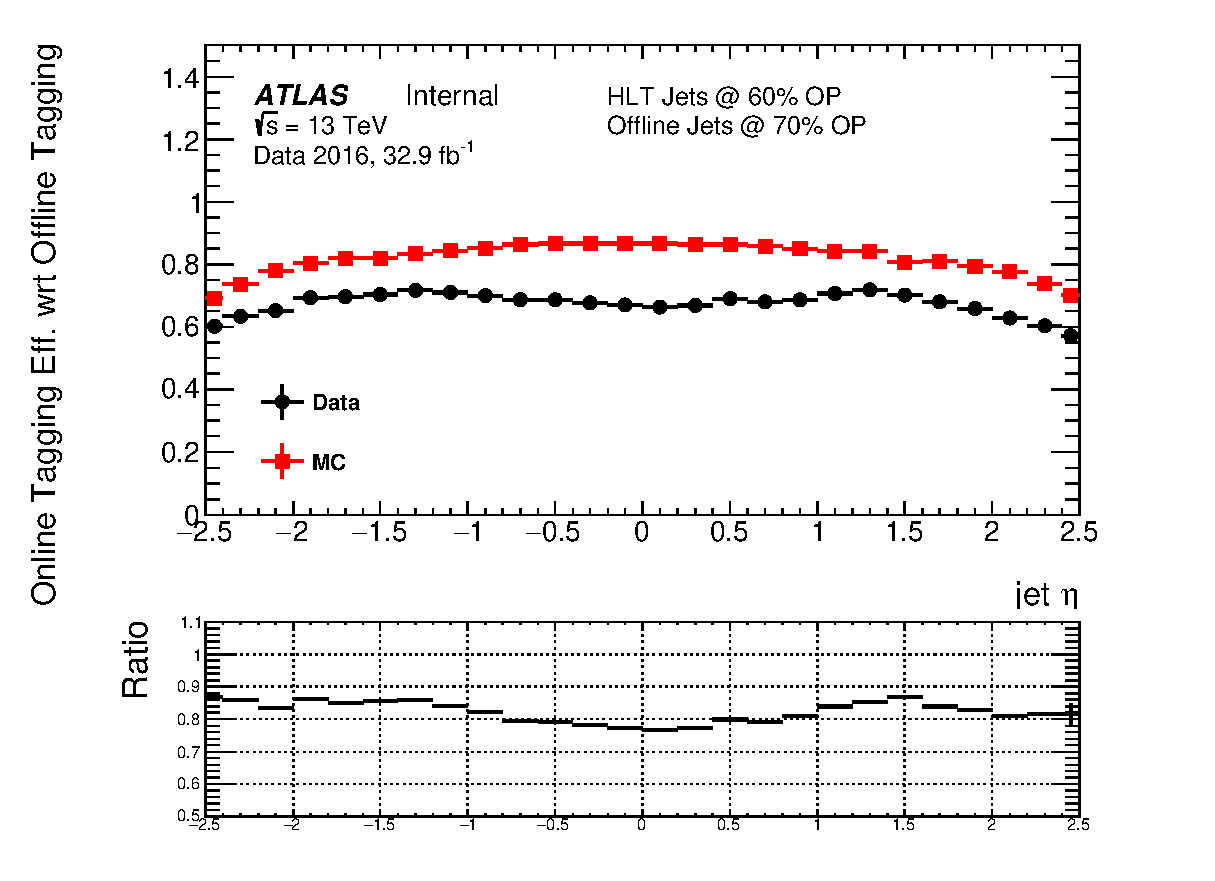
\includegraphics[width=0.48\linewidth, angle=0]{figs/trigger/Full_noGRL_eff_noHLTMatch_jetEta.eps}}
  \end{center}
  \caption[The 60\% $b$-jet trigger efficiency with respect to an offline 70\% operating point tag in Data and simulation
    when the $b$-jet trigger aware GRL is not applied and trigger matching is not required.]
  {The 60\% $b$-jet trigger efficiency with respect to an offline 70\% operating point tag
    for Data (black) and simulation (red) against jet-\pT~(a) and jet-$\eta$ (b).
    The $b$-jet trigger aware GRL is not applied and trigger matching is not required.}
  \label{fig:trig-Full_noGRL_eff_noHLTMatch}
\end{figure}

%\subsection{Investigation}
%\label{sec:trig-inv}

A number of cross-checks were performed to investigate the discrepancy between data and simulation shown in Figure~\ref{fig:trig-Full_noGRL_eff_noHLTMatch}:
including checking for a dependence of the $b$-jet trigger efficiency on the ATLAS detector conditions and number of pile-up collisions.
It has been discovered that the problem causing the large data-simulation discrepancies was related to hard-scatter primary vertex finding.

As described in Section~\ref{sec:trig-bjet}, in 2016 data-taking an algorithm known as \verb|xPrmVtx| is used to find the hard-scatter primary vertex (PV) in the $b$-jet trigger.
It has since been uncovered that there was an error in implementation of this algorithm that depends on the online beam-spot position.
The beam-spot position is defined as the centre of region in the ATLAS detector where the two proton bunches cross,
The beam-spot position is estimated at the trigger-level using the average position of reconsctucted primary verticies over many events,
this is known as the online beam-spot position~\cite{trig-onlinePV}.
Online tracks passed to \verb|xPrmVtx| use positions with respect to the online beam-spot position,
where the \verb|xPrmVtx| algorithm assumed track positions with respect to the origin.
As a result, if the online beamspot $z$-position is far from from the origin then
a valid \verb|xPrmVtx| cannot be found and a dummy PV with position at the origin is passed to the $b$-tagging algorithms
leading to sub-optimal performance. The evidence for this hypothesis is discussed in the remainder of this section.
For brevity, online beamspot $z$-position is henceforth referred to as $z_{\,\text{bs}}^{\text{\,online}}$.  

The exact configuration of the $b$-jet trigger has changed over time to respond to performance issues as they are observed.
The 2016 data is therefore split into 3 different \textit{`epochs'} of data, which are defined by the effect on $b$-jet trigger performance of not finding a valid \verb|xPrmVtx| PV.
The epochs are summarised in Table~\ref{tab:trig-epochs}.
%The relevant conditions of the $b$-jet trigger can be split into three regions of data-taking, which I will refer to as \textit{`epochs'}.
Each epoch is therefore investigated independently.
 
\begin{table}[!htb]
  \begin{center}
  \begin{tabular}{ | c || c | c |}
    \hline			
    \textbf{Epoch}  & \textbf{Integrated Luminosity}    & \textbf{Effect if no \textit{xPrmVtx} PV is found} \\ \hline
    \parbox[c]{0.2cm}{\vspace{0.5em}1}      &  \parbox[c]{1cm}{\vspace{0.5em}~0.8~\ifb{}}     & \parbox[t]{4.5cm} {An invalid primary vertex \\is used in online $b$-tagging. \vspace{0.2em}} \\
    \hline                                                     
    \parbox[c]{0.2cm}{\vspace{0.5em}2}      &  \parbox[c]{1.2cm}{\vspace{0.5em}15.2~\ifb{}}     & \parbox[t]{4.5cm}{The $b$-jet trigger will not \\pass the event. \vspace{0.2em} }\\
    \hline                                                
    \parbox[c]{0.2cm}{\vspace{0.5em}3}      &  \parbox[c]{1cm}{\vspace{0.5em}~8.3~\ifb{}}     & \parbox[t]{4.5cm} {A back-up primary vertex \\ finding algorithm is used.\vspace{0.2em}} \\
    \hline
  \end{tabular}
  \end{center}
  %\vspace{pt}
  \caption{A table summarising the effect of not finding a valid \textit{xPrmVtx} primary vertex in different epochs of data.}
  \label{tab:trig-epochs}
\end{table}

%\begin{table}[!htb]
%  \begin{tabular}{ | c | c | c | c |}
%    \hline			
%    \textbf{Epoch}  & \textbf{Runs}                                  & \textbf{Periods}       & \textbf{Effect if no \textit{xPrmVtx} PV is found} \\ \hline
%      1             & \parbox[t]{2.6cm} {296939-300571,\\ 300655 \\} & A,B(part)              & \parbox[t]{4.5cm} {An invalid primary vertex \\is used in online $b$-tagging.\\ } \\
%    \hline                                                                                                 
%      2             & \parbox[t]{2.6cm} {300600,\\ 300784-308084\\}  & B(part),C,D,E,F,G,I,J  & \parbox[t]{4.5cm} {The $b$-jet trigger is not fired. \\ }\\
%    \hline  
%      3             & \parbox[t]{2.6cm} {309331-311481\\}            & K,L                    & \parbox[t]{4.5cm} {A back-up primary vertex \\ finding algorithm is used.\\} \\
%    \hline
%  \end{tabular}
%  \vspace{10pt}
%  \caption{A table describing the effect of not finding a valid xPrmVtx primary vertex on different epochs of data.}
%  \label{tab:trig-epochs}
%\end{table}
%For Epoch 1, the $\epsilon_{bPerf}$ is 100\% as shown in Figure~\ref{fig:Epoch1_bperf} for Period A.Figure~\ref{fig:Epoch1_eff} shows the $\epsilon_{b\text{Trig}}$ in Epoch 1,

Firstly let us consider Epoch 1;
Figure~\ref{fig:Epoch1_eff}(a) shows that the $b$-jet trigger efficiency against jet-\pT~is ~80-90\% of that in simulation.
Figure~\ref{fig:Epoch1_eff}(b) shows that the $b$-jet trigger efficiency in Epoch 1 has a strong dependence of  $z_{\,\text{bs}}^{\text{\,online}}$;
when $z_{\,\text{bs}}^{\text{\,online}}$ is close to zero the $b$-jet trigger efficiency in data and simulation are comparable
\footnote{In simulation the  $z_{\,\text{bs}}^{\text{\,online}}$ is always set to zero.}
but as $|z_{\,\text{bs}}^{\text{\,online}}|$ increases efficiency falls off steeply.

To understand this performance the variable \textit{`vertex class'} is studied, which is defined as 0 when a valid \verb|xPrmVtx| PV is found and 1 if not.
Figure~\ref{fig:Epoch1_vtxClass}(a) shows that when a \verb|xPrmVtx| PV is found the $b$-jet trigger efficiency is reasonably high ($\sim$ 0.8)
and is comparable between data and simulation (within 5\%),
whilst if no valid \verb|xPrmVtx| PV is found then efficiency is very low in both simulation and data.
However, Figure~\ref{fig:Epoch1_vtxClass}(b) shows that a valid \verb|xPrmVtx| PV is found in simulation for $> 99$ \% of the jets,
whilst in data there is $\sim$ 16\% of events where no valid \verb|xPrmVtx| PV is found.
Hence, combining the information in Table~\ref{tab:trig-epochs}, Figure~\ref{fig:Epoch1_eff} and Figure~\ref{fig:Epoch1_vtxClass}
it can be concluded that for events in  Epoch 1 where the  $|z_{\,\text{bs}}^{\text{\,online}}|$ is far from 0,
the \verb|xPrmVx| returns an dummy vertex which results in a low $b$-jet trigger efficiency.
This is the cause of the data/simulation differences observed in Epoch 1. 


\begin{figure}[!t]
  \begin{center}
    \captionsetup[subfigure]{aboveskip=0pt,justification=centering}
    \subcaptionbox{Jet-\pT}{\includegraphics[width=0.48\linewidth, angle=0]{figs/Trigger/btrigger_old/Epoch1_trigReq_eff_jetPt.pdf} }
    \subcaptionbox{ $z_{\,\text{bs}}^{\text{\,online}}$}{\includegraphics[width=0.48\linewidth, angle=0]{figs/Trigger/btrigger_old/Epoch1_trigReq_eff_bs_online_vz.pdf} }
  \end{center}
  \vspace{-1em}
  \caption[The $b$-jet trigger efficiency with respect to an offline $b$-tagging
    for data from Epoch 1 and simulation against jet-\pT and online beamspot $z$-position.
    The $b$-jet trigger aware GRL has not been applied.]
          {The 60\% $b$-jet trigger efficiency with respect to an offline 70\% operating point tag
            for data from Epoch 1 (black) and simulation (red) against jet-\pT~(a) and online beamspot $z$-position (b).
            The $b$-jet trigger aware GRL has not been applied.}
          \label{fig:Epoch1_eff}
%\end{figure}
%\begin{figure}[!ht]
  \begin{center}
    \captionsetup[subfigure]{aboveskip=0pt,justification=centering}
    \subcaptionbox{$\epsilon_{b\text{Trig}}$ against Vertex Class}{\includegraphics[width=0.48\linewidth, angle=0]{figs/Trigger/btrigger_old/Epoch1_trigReq_eff_vtxClass.pdf}}
    \subcaptionbox{Freq. of Offline Jets against Vertex Class}{\includegraphics[width=0.48\linewidth, angle=0]{figs/Trigger/btrigger_old/Epoch1_trigReq_nOff_vtxClass.pdf}}
  \end{center}
    \vspace{-1em}
  \caption[The $b$-jet trigger efficiency with respect to an offline $b$-tagging
    and  the number of offline jets against vertex class for data from Epoch 1 and simulation.
    The $b$-jet trigger aware GRL has not been applied.]
          {(a) The 60\% $b$-jet trigger efficiency with respect to an offline 70\% operating point tag
    and  (b) the number of offline jets passing 70\% operating point tag and matching a HLT trigger jet
    against vertex class for data from Epoch 1 (black) and simulation (red).
    Vertex class is defined as 0 when a valid \textit{xPrmVtx} vertex is found and 1 if not.
    The $b$-jet trigger aware GRL has not been applied.}
    \label{fig:Epoch1_vtxClass}
\end{figure}


%\begin{figure}[!ht]
%\begin{center}
%  \includegraphics[width=0.47\linewidth, angle=0]{figs/Trigger/btrigger_old/Epoch1_trigReq_bPerfEff_jetPt.pdf}
%  \includegraphics[width=0.47\linewidth, angle=0]{figs/Trigger/btrigger_old/Epoch1_trigReq_bPerfEff_bs_online_vz.pdf}
%\end{center}
%\caption{$b$-performance trigger efficiency, $\epsilon_{bPerf}$, for data from Period A (black) and simulation (red) against jet-pT~(left) and online beamspot $z$-position (right).}
%\label{fig:Epoch1_bperf}
%\end{figure}

In Epoch 2, there is a similar problem to Epoch 1, but there is a subtle difference which requires us to look at this region in a different way.
As in Epoch 1, when  $z_{\,\text{bs}}^{\text{\,online}}$ is far from zero then a \verb|xPrmVtx| PV is not found.
In Epoch 2 if a \verb|xPrmVtx| PV is not found, the $b$-jet trigger procedure falsely terminates whilst processing the event and therefore the trigger does not pass the event.
In addition, $b$-performance triggers will not be passed when no \verb|xPrmVtx| PV is found.
This means that events with no \verb|xPrmVtx| PV are lost in both numerator and denominator when calculated $b$-jet trigger efficiency,
such that the $b$-jet trigger efficiency  should be consistent in data and simulation. 
Figure~\ref{fig:Epoch2_eff} shows that the $b$-jet trigger efficiency measured in data to be in agreement with simulation within 5\%.

For Epoch 2, it is necessary to account for the cases when a \verb|xPrmVtx| PV is not found
by measuring the $b$-performance trigger efficiency, $\epsilon_{bPerf}$,
which is the efficiency that there is a valid primary vertex in the event.
$\epsilon_{bPerf}$ is calculated by dividing the number of events that pass the single muon $b$-performance trigger
by the number of events that pass the equivalent signle muon trigger with no $b$-performance functionality
\footnote{ Specifically $\epsilon_{bPerf}$ = Number of events that pass \textit{HLT\_mu26\_imedium\_2j35\_bperf} divided by the number that pass \textit{HLT\_mu26\_imedium}.}.
The denominator of $\epsilon_{bPerf}$ has no $b$-jet trigger dependency so is unaffected by the \verb|xPrmVtx| algorithm.
$\epsilon_{bPerf}$ is an event level quantity that must be measured with respect to other event level quantities, such as leading jet-\pT.
Figure~\ref{fig:Epoch2_bperf}(a) shows that $\epsilon_{bPerf}$ has a data/simulation ratio of around 80\%  which is similar to that shown in Figure~\ref{fig:Epoch1_eff}.
Figure~\ref{fig:Epoch2_bperf}(b) shows that $\epsilon_{bPerf}$ has a similar shape with respect to  $z_{\,\text{bs}}^{\text{\,online}}$ as observed in Epoch 1,
shown in Figure~\ref{fig:trig-Full_noGRL_eff_noHLTMatch}.

Furthermore in Figure~\ref{fig:Epoch2_bperf}(c) it is shown that $\epsilon_{bPerf}$ has a lower efficiency at smaller values of absolute leading jet-$\eta$.
This shows that the $b$-jet trigger performance problems cause a kinematic bias with respect to leading jet-$\eta$,
an effect that must be accounted for in the final efficiency measurement.

\begin{figure}[!ht]
\begin{center}
  \captionsetup[subfigure]{aboveskip=0pt,justification=centering}
  \subcaptionbox{Jet-\pT}{\includegraphics[width=0.47\linewidth, angle=0]{figs/Trigger/btrigger_old/Epoch2_trigReq_eff_jetPt.pdf}}     
  \subcaptionbox{$z_{\,\text{bs}}^{\text{\,online}}$}{\includegraphics[width=0.47\linewidth, angle=0]{figs/Trigger/btrigger_old/Epoch2_trigReq_eff_bs_online_vz.pdf}}
  %\subcaptionbox{??}{\includegraphics[width=0.47\linewidth, angle=0]{figs/Trigger/btrigger_old/Epoch2_trigReq_eff_jetEta.pdf}} \\
  %\subcaptionbox{??}{\includegraphics[width=0.47\linewidth, angle=0]{figs/Trigger/btrigger_old/Epoch2_trigReq_eff_vtxClass.pdf}}
\end{center}
\caption{The 60\% $b$-jet trigger efficiency with respect to an offline 70\% operating point tag
         for data from Epoch 2 (black) and simulation (red) against jet-\pT~(a), jet-$\eta$ (b) and online beamspot $z$-position.}
\label{fig:Epoch2_eff}
%\end{figure} 
%\begin{figure}[!ht]
\begin{center}
  \captionsetup[subfigure]{aboveskip=0pt,justification=centering}
  \subcaptionbox{Leading jet-\pT}{\includegraphics[width=0.47\linewidth, angle=0]{figs/Trigger/btrigger_old/Epoch2_trigReq_bPerfEff_jetPt.pdf}}
  \subcaptionbox{$z_{\,\text{bs}}^{\text{\,online}}$}{\includegraphics[width=0.47\linewidth, angle=0]{figs/Trigger/btrigger_old/Epoch2_trigReq_bPerfEff_bs_online_vz.pdf}}\\
  \subcaptionbox{Leading jet-$\eta$}{\includegraphics[width=0.47\linewidth, angle=0]{figs/Trigger/btrigger_old/Epoch2_trigReq_bPerfEff_jetEta.pdf}}
\end{center}
\caption{$b$-performance trigger efficiency, $\epsilon_{bPerf}$, for data from Epoch 2 (black) and simulation (red) against (a) leading-jet \pT{}, (b) online beamspot $z$-position
and (c) leading jet-\eta}
\label{fig:Epoch2_bperf}
\end{figure}

%\begin{figure}[!ht]
%\begin{center}
%  \captionsetup[subfigure]{aboveskip=0pt,justification=centering}
%\end{center}
%\caption{$b$-performance trigger efficiency, $\epsilon_{bPerf}$, for data from Epoch 2 (black) and simulation (red) against leading-jet \eta{}.}
%\label{fig:Epoch2_bperf_eta}
%\end{figure}

For Epoch 3, when no \verb|xPrmVtx| PV is found a backup PV finding algorithm is used.
The backup algorithm is \verb|EFHist|, which finds the PV through a basic histogramming of the tracks.
The simplicity of the \verb|EFHist| algorithm means that a PV can be found as long as 1 track is present.
Figure~\ref{fig:Epoch3_eff} shows the $b$-jet trigger efficiency in Epoch 3 for jet-\pT, jet-$\eta$,  $z_{\,\text{bs}}^{\text{\,online}}$ and vertex class (as defined above).
In Epoch 3 the $b$-jet trigger efficiency measured in data is within 5\% of simulation and there is no shape difference between the two with respect to jet-$\eta$.
In addition it is shown that in Epoch 3 there is no strong dependence on  $z_{\,\text{bs}}^{\text{\,online}}$,
and that efficiency in data is consistent if a valid \verb|xPrmVtx| PV is found or not (vertex class = 0 or 1 respectively).
This demonstrates that the use of backup finding algorithm alleviates the $b$-jet trigger performance observed in Epoch 1 and Epoch 2.

\begin{figure}[!htb]
\begin{center}
  \captionsetup[subfigure]{aboveskip=0pt,justification=centering}
  \subcaptionbox{Jet-\pT}{\includegraphics[width=0.47\linewidth, angle=0]{figs/Trigger/btrigger_old/Epoch3_trigReq_eff_jetPt.pdf}}
  \subcaptionbox{Jet-$\eta$}{\includegraphics[width=0.47\linewidth, angle=0]{figs/Trigger/btrigger_old/Epoch3_trigReq_eff_jetEta.pdf}} \\
  \subcaptionbox{$z_{\,\text{bs}}^{\text{\,online}}$}{\includegraphics[width=0.47\linewidth, angle=0]{figs/Trigger/Epoch3_eff_bs_online_vz.eps}}
  \subcaptionbox{Vertex Class}{\includegraphics[width=0.47\linewidth, angle=0]{figs/Trigger/btrigger_old/Epoch3_trigReq_eff_vtxClass.pdf}}
\end{center}
%\caption{The 60\% $b$-jet trigger efficiency with respect to an offline 70\% operating point tag
%  for data from Epoch 3 (black) and simulation (red) against (a) jet-\pT and (b) vertex class.
%  Vertex class is defined as 0 when a valid \textit{xPrmVtx} vertex is found and 1 if not.
%}
\caption{The 60\% $b$-jet trigger efficiency with respect to an offline 70\% operating point tag
  for data from Epoch 3 (black) and simulation (red) against (a) jet-\pT, (b) jet-$\eta$,
  (c) online beamspot $z$-position and (d) vertex class.}
\label{fig:Epoch3_eff}
\end{figure}

\newpage
\subsection{Solution: $b$-Jet Trigger GRL}
\label{sec:trig-grl}

To summarise, in the previous section it is shown that at large values of absolute online beamspot $z$-position
the measured $b$-jet trigger efficiency in Epoch 1 and $\epsilon_{bPerf}$ in Epoch 2 is lower in data than in simulation
due to poor \verb|xPrmVtx| PV finding performance.
In Epoch 3 there is reasonable data/simulation agreement due to the use of a backup vertex finding algorithm. 

To resolve the large data-simulation discrepancies a $b$-jet trigger aware GRL is applied
to remove events with $|z_{\,\text{bs}}^{\text{\,online}}| >$ 2mm in Epoch 1 and 2,
such that the events with low efficiency are removed.
To retain as much data as possible, the cut value is chosen be the widest value of $|z_{\,\text{bs}}^{\text{\,online}}|$
that corresponds to an efficiency not significantly reduced by the \verb|xPrmVtx| algorithm performance issue.
A \SI{2}{\mm} cut is selected using Figure~\ref{fig:Epoch1_eff}(b) and Figure~\ref{fig:Epoch2_bperf}(b).

It was decided to use a $b$-jet trigger aware GRL instead of deriving a correction factor for the full data-set.
The cost of using a $b$-jet trigger aware GRL is a reduction in the integrated luminosity of the data-set from  32.9~\ifb{} to 24.3~\ifb.
The reasons for using a $b$-jet trigger aware GRL are threefold.
Firstly, as there is no beamspot position distribution in simulation it is not clear that kinematics of events at high  $z_{\,\text{bs}}^{\text{\,online}}$ can be well understood and modelled;
the sculpting of the efficiency with respect to jet-$\eta$ shown in Figure~\ref{fig:Epoch2_bperf}(c) is an example of this.
Secondly, the efficiencies are quite low at high beamspot $z$-position,
so the loss in luminosity x acceptance is relatively small.
Finally, using a GRL means that the stated value of integrated luminosity is a more accurate representation of the number collisions considered.

After the GRL is applied, the $b$-jet trigger efficiency for Epoch 1 becomes approximately 90-95\% of the efficiency measured in simulation,
as shown in Figure~\ref{fig:Epoch1_bslt2mm_eff}.
Similarly, after the $b$-jet trigger aware GRL is applied, $\epsilon_{bPerf}$ for Epoch 2 becomes approximately 95\% of the efficiency measured in simulation,
as shown in Figure~\ref{fig:Epoch2_bslt2mm_bperf}. 

\begin{figure}[!ht]
  \begin{center}
    \captionsetup[subfigure]{aboveskip=0pt,justification=centering}
    \subcaptionbox{Jet-\pT}{\includegraphics[width=0.47\linewidth, angle=0]{figs/Trigger/btrigger_old/Epoch1_GRL_bslt2mm_trigReq_eff_jetPt.pdf} }
    \subcaptionbox{Jet-$\eta$}{\includegraphics[width=0.47\linewidth, angle=0]{figs/Trigger/btrigger_old/Epoch1_GRL_bslt2mm_trigReq_eff_jetEta.pdf}}
  \end{center}
  \caption{The 60\% $b$-jet trigger efficiency with respect to an offline 70\% operating point tag
    for data from Epoch 1 (black) and simulation (red) against jet-\pT~(a) and jet-$\eta$ (b).
    The $b$-jet trigger aware GRL has been applied.}
  \label{fig:Epoch1_bslt2mm_eff}
\end{figure}

\begin{figure}[!ht]
  \begin{center}
    \captionsetup[subfigure]{aboveskip=0pt,justification=centering}
    \subcaptionbox{Leading jet-\pT}{\includegraphics[width=0.47\linewidth, angle=0]{figs/Trigger/btrigger_old/Epoch2_GRL_bslt2mm_trigReq_bPerfEff_jetPt.pdf} }
    \subcaptionbox{Leading jet-$\eta$}{\includegraphics[width=0.47\linewidth, angle=0]{figs/Trigger/btrigger_old/Epoch2_GRL_bslt2mm_trigReq_bPerfEff_jetEta.pdf}}
  \end{center}
  \caption{$b$-performance trigger efficiency, $\epsilon_{bPerf}$, for data from Epoch 2 (black) and simulation (red) against leading (a) jet-\pT~and (b) jet-$\eta$.
    The $b$-jet trigger aware GRL has been applied.}
  \label{fig:Epoch2_bslt2mm_bperf}
\end{figure}

Figures~\ref{fig:Full_bslt2mm_eff} and ~\ref{fig:Full_bslt2mm_bperf} shows the measured
$b$-jet trigger efficiency and $\epsilon_{bPerf}$
for the full 2016 data-set, combining Epochs 1, 2 and 3,
with the $b$-jet trigger aware GRL applied.
%This represents the raw observed data/simulation efficiencies when the full event selection has been applied.

\begin{figure}[!ht]
  \begin{center}
    \captionsetup[subfigure]{aboveskip=0pt,justification=centering}
    \subcaptionbox{Jet-\pT}{\includegraphics[width=0.47\linewidth, angle=0]{figs/Trigger/btrigger_old/Full_GRL_bslt2mm_trigReq_eff_jetPt.pdf}}
    \subcaptionbox{Jet-$\eta$}{\includegraphics[width=0.47\linewidth, angle=0]{figs/Trigger/btrigger_old/Full_GRL_bslt2mm_trigReq_eff_jetEta.pdf}}\\
    \subcaptionbox{$z_{\,\text{bs}}^{\text{\,online}}$}{\includegraphics[width=0.47\linewidth, angle=0]{figs/Trigger/btrigger_old/Full_GRL_bslt2mm_trigReq_eff_bs_online_vz.pdf}}
    \subcaptionbox{Vertex Class}{\includegraphics[width=0.47\linewidth, angle=0]{figs/Trigger/btrigger_old/Full_GRL_bslt2mm_trigReq_eff_vtxClass.pdf}}
  \end{center}
  \caption{The 60\% $b$-jet trigger efficiency with respect to an offline 70\% operating point tag
    for the full 2016 data-set (black) and simulation (red) against jet-\pT~(a), jet-$\eta$ (b), online beamspot $z$-position (c) and vertex class (d).
    Vertex class is defined as 0 when a valid \textit{xPrmVtx} vertex is found and 1 if not.
}
  \label{fig:Full_bslt2mm_eff}
\end{figure}

%\begin{figure}[!ht]
%  \begin{center}
%    \captionsetup[subfigure]{aboveskip=0pt,justification=centering}
%    \subcaptionbox{Jet-\pT}{\includegraphics[width=0.47\linewidth, angle=0]{figs/Trigger/btrigger_old/Full_GRL_bslt2mm_trigReq_eff_jetPt.pdf}}
%    \subcaptionbox{Jet-$\eta$}{\includegraphics[width=0.47\linewidth, angle=0]{figs/Trigger/btrigger_old/Full_GRL_bslt2mm_trigReq_eff_jetEta.pdf}}\\
%    \subcaptionbox{$z_{\,\text{bs}}^{\text{\,online}}$}{\includegraphics[width=0.47\linewidth, angle=0]{figs/Trigger/btrigger_old/Full_GRL_bslt2mm_trigReq_eff_bs_online_vz.pdf}}
%    \subcaptionbox{Vertex Class}{\includegraphics[width=0.47\linewidth, angle=0]{figs/Trigger/btrigger_old/Full_GRL_bslt2mm_trigReq_eff_vtxClass.pdf}}
%  \end{center}
%  \caption{The 60\% $b$-jet trigger efficiency with respect to an offline 70\% operating point tag
%    for the full 2016 data-set (black) and simulation (red) against jet-\pT~(a), jet-$\eta$ (b), online beamspot $z$-position (c) and vertex class (d).}
%  \label{fig:Full_bslt2mm_eff}
%\end{figure}

\begin{figure}[!ht]
  \begin{center}
    \captionsetup[subfigure]{aboveskip=0pt,justification=centering}
    \subcaptionbox{Leading jet-\pT}{\includegraphics[width=0.47\linewidth, angle=0]{figs/Trigger/btrigger_old/Full_GRL_bslt2mm_trigReq_bPerfEff_jetPt.pdf}}
    \subcaptionbox{Leading jet-$\eta$}{\includegraphics[width=0.47\linewidth, angle=0]{figs/Trigger/btrigger_old/Full_GRL_bslt2mm_trigReq_bPerfEff_jetEta.pdf}}
  \end{center}
  \caption{$b$-performance trigger efficiency, $\epsilon_{bPerf}$, for the full 2016 data-set (black) and simulation (red) against (a) leading jet-\pT~and (b) jet-$\eta$.
    The $b$-jet trigger aware GRL has been applied.}
  \label{fig:Full_bslt2mm_bperf}
\end{figure}
  

\FloatBarrier
\newpage

\subsection{Efficiency Measurement and Associated Uncertainties}
\label{sec:trig-eff_syst}

In the previous two sections it has been shown that when applying a $b$-jet aware GRL,
the $b$-jet trigger performance is understood and the data/simulation agreement is within 5\%.
The remaining data/simulation differences are accounted for using a data/simulation scale factor.
This section presents the measurement of the data/simulation scale factors (SFs) (defined in Section~\ref{sec:trig-bjet_strat})
and the derivation of the associated uncertainties.
In this section the full 2016 data set is used
and the full event selection from Section~\ref{sec:trig-evtSel} is applied.

As discussed above, there are two factors considered in this section.
Firstly there is the $b$-jet trigger efficiency measurement
that accounts for differences in online and offline $b$-tagging given that a valid primary vertex has been found.
Sections~\ref{sec:trig-purity}~to~\ref{sec:trig-highPtExtrap} describe the derivation of a set of systematic uncertainties and corrections to the raw measurement
and Section~\ref{sec:trig-jetLevelEff} presents the final measurement.
The $b$-jet trigger efficiency scale factor is applied as a jet-level correction to simulation.
Secondly, in Section~\ref{sec:trig-eventLevelEff}, is a description the measurement of the $\epsilon_{bPerf}$ and the relevant systematic uncertainties,
that accounts for the efficiency of finding a valid primary vertex.
$\epsilon_{bPerf}$ is applied to the simulation as an event level efficiency.

% This section got cut and moved to jetLevelEff
%\subsubsection{$\eta$ Dependence on Efficiency}
%\label{sec:trig-etaDep}
%\begin{figure}[!ht]
%  \begin{center}
%    \includegraphics[width=0.47\linewidth, angle=0]{figs/Trigger/btrigger_old/Full_GRL_bslt2mm_trigReq_eff_jetPt.pdf}
%    \includegraphics[width=0.47\linewidth, angle=0]{figs/Trigger/btrigger_old/Full_GRL_bslt2mm_trigReq_eff_jetEta.pdf}
%  \end{center}
%  \caption{The 60\% $b$-jet trigger efficiency with respect to an offline 70\% operating point tag
%    for data from Periods A-L (black) and simulation (red) against jet-\pT~(a), jet-$\eta$ (b).}
%  \label{fig:Full_bslt2mm_eff_eta}
%\end{figure}

\subsubsection{Purity Uncertainty}
\label{sec:trig-purity}

It is known that despite the strict event selection there will inevitably be non $b$-jet contamination included in the calculation of $b$-jet trigger efficiencym
to estimate the size of the non-$b$-jet contamination simulation is used.

In simulation a jet is categorised as a true $b$-jet, a true $c$-jet or a true light-jet;
the truth labelling scheme used is described in Section~\ref{sec:obj-bjets_label}.
For this measurement true $c$ and light jets are grouped together in a non-$b$-jet category.
The superset of jets with no truth flavour categorisation applied are referred to as inclusive jets.

The $b$-jet purity is defined as the fraction of jets used in the $b$-jet trigger efficiency calculation that are true $b$-jets.
Figure~\ref{fig:Purity} shows the number of true $b$-jets and number of inclusive jets that are tagged at the 70\% operating point as a function of jet-\pT~and jet-$\eta$;
the lower panel shows ratio of the two, which is the $b$-jet purity.
The $b$-jet purity is $>$ 95\% up to jet-\pT$\sim$300~\GeV~and $>$ 90\% for higher values of jet-\pT.

A purity correction to the $b$-jet trigger efficiency to account for the non-$b$-jet contanination is derived using simulation.
An uncertainty on the modelling of the non-$b$-jet contanination is derived by varying the size of the non-$b$-jet contamination in simulation.
Figure~\ref{fig:Eff_Purity}(a) shows the $b$-jet efficiency for inclusive jets, true-$b$-jets and true non-$b$-jets.
The ratio of the efficiency for only true $b$-jets and inclusive jets is shown in the lower panel,
this ratio is applied to the measured $b$-jet efficiency as the purity correction.
Figure~\ref{fig:Eff_Purity}(b) shows the $b$-jet efficiency for inclusive jets and the case when the non-$b$-jet contamination has been doubled,
the ratio is shown in the lower panel.
The maximum difference from the efficiency measured for the inclusive jets and the cases
where there is only true $b$-jets and where the non $b$-jet content has been doubled,
shown in the two ratio plots in Figure~\ref{fig:Eff_Purity}, is taken as symmetric uncertainty.

\begin{figure}[!ht]
  \begin{center}
    \captionsetup[subfigure]{aboveskip=0pt,justification=centering}
    \subcaptionbox{Jet-\pT}{\includegraphics[width=0.47\linewidth, angle=0]{figs/Trigger/btrigger_old/PurityMC_jetPt.pdf}}
    \subcaptionbox{Jet-$\eta$}{\includegraphics[width=0.47\linewidth, angle=0]{figs/Trigger/btrigger_old/PurityMC_jetEta.pdf}}
  \end{center}
  \caption{A comparison of the number of offline jets tagged at the 70\% operating point
    for inclusive jets (red) and truth-matched $b$-jets (blue)
    against jet-\pT~(a) and jet-$\eta$ (b) in a simulated sample.}
  \label{fig:Purity}
\end{figure}

\begin{figure}[!ht]
  \begin{center}
    \captionsetup[subfigure]{aboveskip=0pt,justification=centering}
    \subcaptionbox{}{\includegraphics[width=0.47\linewidth, angle=0]{figs/Trigger/btrigger_old/EffMC_jetPt_trueB.pdf}}
    \subcaptionbox{}{\includegraphics[width=0.47\linewidth, angle=0]{figs/Trigger/btrigger_old/EffMC_jetPt_2nonB.pdf}}
  \end{center}
  \caption{The 60\% $b$-jet trigger efficiency with respect to an offline 70\% operating point tag
    for inclusive jets (black) compared to truth matched $b$-jets and non $b$-jets (a) and the case where non $b$-jet content has been doubled (b) for a simulated $t\bar{t}$ sample.
    The lower panel in both plots show the ratio to the inclusive efficiency.
  }
  \label{fig:Eff_Purity}
\end{figure}

\subsubsection{Non-$b$-jet trigger efficiency uncertainty}
\label{sec:trig-lightTrigEff}

As one would expect and as shown in left plot of Figure~\ref{fig:Eff_Purity}, non $b$-jets (shown in blue) have a different $b$-jet trigger efficiency to that of $b$-jets.
However the exact efficiency is not known well and could be mismodelled in simulation.
To account for this uncertainty the nominal efficiency in simulation is compared
to the cases where the non-$b$-jet efficiency has been halved and doubled in simulation, as shown in Figure~\ref{fig:Eff_LTrigEff}.
When doubling the non-$b$-jet trigger efficiency this is limited at the upper end to being no greater than the true $b$-jet trigger efficiency.
The maximum bin-by-bin difference between the nominal and the two cases, as shown in the two ratio plots, is taken as a symmetric systematic uncertainty.

\begin{figure}[!ht]
  \begin{center}
    \captionsetup[subfigure]{aboveskip=0pt,justification=centering}
    \subcaptionbox{}{\includegraphics[width=0.47\linewidth, angle=0]{figs/Trigger/btrigger_old/effMC_jetPt_lowLTrigEff.pdf}}
    \subcaptionbox{}{\includegraphics[width=0.47\linewidth, angle=0]{figs/Trigger/btrigger_old/effMC_jetPt_upLTrigEff.pdf}}
  \end{center}
  \caption{The 60\% $b$-jet trigger efficiency with respect to an offline 70\% operating point tag
    for nominal inclusive case (black) compared to varied inclusive case (red) and just non $b$-jets (blue)
    in the case where non $b$-jet efficiency has been halved (a) and doubled (b) for a simulated $t\bar{t}$ sample.
    The lower panel in both plots show the ratio of the varied inclusive efficiency to the nominal inclusive efficiency.
  }
  \label{fig:Eff_LTrigEff}
\end{figure}

\FloatBarrier

\subsubsection{High-\pT~extrapolation}
\label{sec:trig-highPtExtrap}

Measuring $b$-jet trigger efficiency for high-\pT~jets is limited by the statistics in the simulated $t\bar{t}$ sample,
so the shape from simulation will be used to extrapolate the efficiency for jet-\pT{} $>$ 240 GeV.
The point from which to extrapolate from was chosen as this is when data statistic uncertainty starts to become large. 

The procedure is made of two sequential fits (normalisation and correction) to the data/simulation ratio,
which are used to create a ``corrected simulation'' $b$-jet trigger efficiency distribution.
For jet-$pT$ $>$ 240 GeV, the corrected $b$-jet trigger efficiency is used in place of data when measuring the efficiency in data 
and when calculating data/MC scale factors.
A final quadratic fit is used to assign a systematic uncertainty. 

\noindent
In more detail:
\begin{itemize}
  \setlength\itemsep{1em}
\item \textbf{Flat Normalisation Fit}: \\
  The measured $b$-jet trigger efficiency, in both data and simulation are compared,
  and a horizontal fit is performed to the ratio of the two.
  The fit range is set at $\pT{} > 50\GeV$ to discount the first bin, which has a larger purity uncertainty.
  This is then used to normalise the simulated efficiency distribution to match data.
  This fit is shown in the lower plot  of panel (a) in Figure~\ref{fig:bTrig_mcExtrap}.
  The uncertainty on the one parameter of this fit is taken as a systematic uncertainty.
  
\item \textbf{Linear Correction Fit}:  \\
  The measured $b$-jet trigger efficiency, in both data and the normalised simulation are compared,
  and a linear fit is performed to the ratio of the two from jet-\pT{} $>$ 240 GeV.
  This is then used to correct the simulated efficiency distribution to match data.
  This fit is shown in the lower plot of panel (b) in Figure~\ref{fig:bTrig_mcExtrap}.
  The simulated $b$-jet trigger efficiency, after both the normalisation and linear correction is referred to as the corrected simulation.
  To assign a systematic uncertainty on the fit parameters, the slope of this fit is varied up and down within uncertanties,
  whilst the point at which the fit crosses 1 is kept constant.
  The maximum difference between the nominal fit and the varied fits is taken as the uncertainty on the linear correction fit.
  Panel (c) of Figure~\ref{fig:bTrig_mcExtrap} shows the data compared to the corrected simulation.
  The lower panel shows the ratio of the two, and the blue lines represent the uncertanties on the linear correction fit.
  
\item \textbf{Quadratic Systematic Fit}: \\
  Finally to assess an uncertainty on the choice of a linear fit as the functional form above,
  a fit is performed to the data and corrected simulation ratio using a quadratic function.
  This ratio and the fit is shown in panel (d) of Figure~\ref{fig:bTrig_mcExtrap}.
  The difference of the fit from 1 is considered as the functional form uncertainty when assigning as systematic uncertainty.
  
\end{itemize}

The systematic uncertainty on the extrapolation is defined as the uncertainty from normalisation fit
added to the bin-by-bin maximum of the uncertainty from the linear correction fit and the uncertainty from the quadratic systematic fit.
The uncertanties on the high-\pT~extrapolation procedure are summarised in Table~\ref{tab:bTrig_extrapSyst}
  
\begin{figure}[!ht]
\begin{center}
\captionsetup[subfigure]{aboveskip=0pt,justification=centering}
  \subcaptionbox{Data/MC with normalisation fit} {\includegraphics[width=0.47\linewidth, angle=0]{figs/Trigger/btrigger_old/Full_GRL_bslt2mm_trigReq_effFit_jetPt.pdf} }
  \subcaptionbox{Data/normalised MC with linear correction fit} {\includegraphics[width=0.47\linewidth, angle=0]{figs/Trigger/btrigger_old/Full_GRL_bslt2mm_trigReq_effNormFit_jetPt.pdf}} \\
  \subcaptionbox{Data/corrected MC with linear correction fit uncertanties} {\includegraphics[width=0.47\linewidth, angle=0]{figs/Trigger/btrigger_old/Full_GRL_bslt2mm_trigReq_effCorrShapeErr_jetPt.pdf}}
  \subcaptionbox{Data/corrected MC with quadratic fit } {\includegraphics[width=0.47\linewidth, angle=0]{figs/Trigger/btrigger_old/Full_GRL_bslt2mm_trigReq_effCorrFitQuad_jetPt.pdf}}
\end{center}
\caption{A figure to demonstrate the high-\pT~extrapolation procedure for the 60\% $b$-jet trigger efficiency with respect to an offline 70\% operating point tag.
  Data (black) is compared against simulation (red) after various corrections have been applied  as a function of jet-\pT.
  Panel (a) shows the flat normalisation fit uncorrected simulation, panel (b) shows the linear correction fit to normalised simulation,
  panel (c) shows the linear correction fit uncertanties to the corrected simulation and panel (d) shows the quadratic fit to the corrected simulation.
  }
\label{fig:bTrig_mcExtrap}
\end{figure}

\begin{table}[!ht]
\begin{tabular}{|c||c||c|c|c|c|}
  \hline
  Jet pT [GeV] & MC Extrap. (\%) & Norm Fit (\%) & Lin. Fit (\%) & Quad. Fit (\%)\\
  \hline
  240.0-300.0 & 0.8 & 0.0  & 0.8 & 0.3\\
  300.0-400.0 & 4.0 & 0.0  & 2.9 & 4.0\\
  400.0-500.0 & 5.6 & 0.0  & 5.6 & 1.7\\
  500.0-700.0 & 18.0 & 0.0 & 9.6 & 18.0\\
  \hline
\end{tabular}
  \vspace{10pt}
\caption{A table showing the systematic uncertainty assigned for the high-\pT~extrapolation.}
\label{tab:bTrig_extrapSyst}
\end{table}

\FloatBarrier


\subsubsection{Jet-Level Efficiency and Scale Factor Measurement}
\label{sec:trig-jetLevelEff}

Now the raw measurements of the $b$-jet trigger efficiency from Figure~\ref{fig:Full_bslt2mm_eff}
and the additional corrections and systematic uncertainties described above can be brought together.
In Figure~\ref{fig:Full_bslt2mm_eff} it is shown that, whilst efficiency does depend on jet-$\eta$,
the data to simulation ratio is flat with respect to jet-$\eta$.
However there is no significant dependence on jet-\pT~hence data/simulation scale factors are derived as a function of only jet-\pT. 

The full jet-level $b$-jet trigger efficiency measurement is shown in Figure~\ref{fig:bTrig_jetSys_eff}.
For use in combination with the simulation, a data/simulation scale factor as a
function of jet-\pT~is also derived and will be applied at the jet-level, which is also shown in Figure~\ref{fig:bTrig_jetSys_SF}.

The uncertanties considered for the jet-level efficiency account for:
mismodelling of the $b$-jet purity in simulation, mismodelling of the $b$-jet trigger efficiency for non $b$-jets,
simulation statistical uncertainty , data statistical uncertainty (jet-$p_T <$ 240 \GeV) and simulation based extrapolation (jet-$p_T >$ 240 \GeV).
Table~\ref{tab:bTrig_jetSys} summarises the uncertanties on the jet-level scale factor.
These uncertanties are taken as a symmetric uncertainty in each jet-\pT~bin and the scale factors are applied to each b-tagged jet.\\

As a final sanity check Figure~\ref{fig:bTrig_jetSys_effComp} shows the $b$-jet trigger efficiency measured in data to
that from the corrected simulation, in the lower panel a ratio of data to corrected simulation is shown
and the extrapolation and total uncertanties are overlaid in red and green respectively.
The derivation of the corrected simulation and associated extrapolation uncertanties is described in Section~\ref{sec:trig-highPtExtrap}
This shows that the corrected simulation lies within the total uncertanties for the whole range of jet-\pT~
and at high-\pT, as one might expect, the uncertainty is dominated by the extrapolation uncertainties.
Note that the corrected simulation is only used to represent data for jet-\pT{} $>$ 240 \GeV.

\begin{figure}[!ht]
  \begin{center}
    \includegraphics[width=0.8\linewidth, angle=0]{figs/Trigger/btrigger_old/fullSyst_Efficiency_jetPt.pdf}
  \end{center}
  \caption{
    The measured 60\% $b$-jet trigger efficiency with respect to an offline 70\% operating point tag
    as measured in data as a function of offline jet-\pT.
    The central values are shown in black with the statistical uncertainty and the green bands represent the total uncertainty including systematic uncertanties.
    \label{fig:bTrig_jetSys_eff}
  }
  \begin{center}
    \includegraphics[width=0.8\linewidth, angle=0]{figs/Trigger/btrigger_old/fullSyst_ScaleFactor_jetPt.pdf}
  \end{center}
  \caption{
    Data/simulation scale factors for the 60\% $b$-jet trigger efficiency with respect to an offline 70\% operating point tag
    as a function of offline jet-\pT.
    The central values are shown in black with the statistical uncertainty and the green bands represent the total uncertainty including systematic uncertanties.
    \label{fig:bTrig_jetSys_SF}
  }
\end{figure}

\begin{table}[!ht]
  \begin{tabular}{|c||c|c||c|c|c|c|}
    \hline
    Jet $p_T$ [GeV] & SF & Total Err. (\%) & Stat. (\%) & Extrap. (\%) & Pur. (\%) & L. Trig. Eff. (\%)\\
    \hline
    35.0-50.0 & 95.9 & 1.0 & 0.1 & - & 0.7 & 0.7\\
    50.0-70.0 & 96.8 & 0.7 & 0.1 & - & 0.5 & 0.5\\
    70.0-90.0 & 96.9 & 0.6 & 0.1 & - & 0.5 & 0.5\\
    90.0-120.0 & 96.9 & 0.7 & 0.1 & - & 0.5 & 0.5\\
    120.0-150.0 & 96.7 & 0.6 & 0.2 & - & 0.4 & 0.4\\
    150.0-180.0 & 96.6 & 0.9 & 0.2 & - & 0.6 & 0.6\\
    180.0-240.0 & 95.7 & 1.1 & 0.5 & - & 0.7 & 0.7\\
    \hline
    240.0-300.0 & 95.3 & 2.6 & 0.4 & 0.8 & 1.8 & 1.7\\
    300.0-400.0 & 92.4 & 5.6 & 1.1 & 4.0 & 2.8 & 2.5\\
    400.0-500.0 & 88.8 & 8.1 & 2.6 & 5.6 & 4.2 & 3.3\\
    500.0-700.0 & 83.4 & 19.4 & 4.0 & 18.0 & 4.9 & 3.1\\
    \hline
\end{tabular}
  \caption{A table showing the jet-level Data/simulation scale factor (SF) as a function of jet-$p_{T}$
    with total uncertainty and the contributions of the different uncertainties considered;
    specifically statistical, high-\pT~extrapolation, non-$b$-jet purity and non-$b$-jet trigger efficiency.}
\label{tab:bTrig_jetSys}
\end{table}

\begin{figure}[!ht]
  \begin{center}
    \includegraphics[width=0.8\linewidth, angle=0]{figs/Trigger/fullSys_EfficiencyComp_jetPt.eps}
  \end{center}
  \caption{
    The measured 60\% $b$-jet trigger efficiency with respect to an offline 70\% operating point tag
    as measured in data (black) and from the corrected simulation (red) as a function of offline jet-\pT.
    In the ratio plot on the lower panel the extrapolation uncertanties is represented by the red band, whilst the total uncertainty is overlaid in green.
    \label{fig:bTrig_jetSys_effComp}
  }
\end{figure}

Only the 70\% offline operating point has been shown as this is offline operating points used in the di-$b$-jet analysis (further details are in described in Chapter~\ref{evt}).
However, the jet-level efficiencies and uncertainties are also be calculated all combination other offline operating points.
Table~\ref{tab:trig-bTrig_jetSys_opComp} shows a comparison of the jet level uncertainties for the 70\%, 77\% and 85\% operating point.
This shows that for looser offline operating points the uncertainty becomes larger, due to increased non-$b$-jet impurities.


\begin{table}[ht]
  \begin{center}
  \begin{tabular}{|c||c|c|c|}
    \hline
    \multirow{2}{*}{Jet $p_T$ [GeV]} &\multicolumn{3}{c|}{Systematic Uncertainty for Offline OP} \\ \cline{2-4} 

                & \hspace{1.5mm}70\% OP\hspace{1.5mm} & \hspace{1.5mm}77\% OP\hspace{1.5mm} & \hspace{1.5mm}85\% OP\hspace{1.5mm} \\
    \hline
    35.0-50.0   & 1.0\%   & 2.3\%   & 6.2\%  \\
    50.0-70.0   & 0.7\%   & 1.6\%   & 4.6\%  \\
    70.0-90.0   & 0.6\%   & 1.3\%   & 3.7\%  \\
    90.0-120.0  & 0.7\%   & 1.3\%   & 3.7\%  \\
    120.0-150.0 & 0.6\%   & 1.4\%   & 3.7\%  \\
    150.0-180.0 & 0.9\%   & 1.8\%   & 4.6\%  \\
    180.0-240.0 & 1.1\%   & 2.6\%   & 6.4\%  \\
    \hline          
    240.0-300.0 & 2.6\%   & 4.4\%   & 10.2\% \\
    300.0-400.0 & 5.6\%   & 7.5\%   & 17.6\% \\
    400.0-500.0 & 8.1\%   & 10.9\%  & 22.2\% \\
    500.0-700.0 & 19.4\%  & 19.0\%  & 36.6\% \\
    \hline
  \end{tabular}
  \vspace{10pt}
  \end{center}
  \caption{
    A comparison of the systematic uncertainty on the $b$-jet trigger jet-level efficiency 
    for various offline operating points (OP) w.r.t. the 60\% online operating point.
    The increase in systematic uncertainty for looser offline operating points is driven by non $b$-jet impurities.
  }
  \label{tab:trig-bTrig_jetSys_opComp}
  \end{table}

\FloatBarrier
\newpage

\subsubsection{Event-Level Efficiency and Uncertainties}
\label{sec:trig-eventLevelEff}

As alread discussed, in some regions of data-taking the performance
$b$-jet trigger efficiency itself
depends on the online beamspot position.
Hence, a $b$-jet trigger aware GRL is applied to remove a large fraction of
events where poor $b$-jet trigger performance is observed.

However, even after the application of this GRL,
there remains a bias with respect to leading jet-$\eta$ in the
probability of finding a valid primary vertex, which is notated as $\epsilon_{bPerf}$.
This bias is shown in Figure~\ref{fig:Full_bslt2mm_bperf}.
This efficiency is measured differently in each epoch,
in Epoch 1 it can be found as the number of events with vertex class = 0 divided by the number of events,
in Epoch 2 it is defined as the dividing the number of events that pass the trigger
\verb|HLT_mu26_imedium_2j35_bperf| by the number that pass the trigger \verb|HLT_mu26_imedium|
and in Epoch 3, due to the back-up vertex.
It should be noted that this measurement made in each of the three regions separately and is then combined with each region weighted by its luminosity.

The value of $\epsilon_{bPerf}$ is extremely close to 1 in simulation, in this case the efficiency in data and the scale factor are the same.
To assign a systematic uncertainty for this correction the statistical uncertainty in data and simulation in addition to a shape systematic uncertainty are used.
The shape systematic uncertainty, to account for possible variations of the shape with respect to jet-$\eta$,
is defined as half of the difference between the maximum efficiency and the minimum efficiency in any jet-$\eta$ bin,
which effectively covers a flat distribution with respect to jet-$\eta$ to one where the shape is twice is extreme as observed.

Table~\ref{tab:bTrig_eventEff} and Figure~\ref{fig:bTrig_eventSys}
summarises the event-level efficiency correction and the associated systematic uncertainties.

\begin{figure}[!ht]
  \begin{center}
    \includegraphics[width=0.8\linewidth, angle=0]{figs/Trigger/btrigger_old/fullSyst_EventEfficiency_leadingJetEta.pdf}
  \end{center}
  \caption{
    The measured $\epsilon_{bPerf}$ as measured in data as a function of offline leading jet-$\eta$.
    The central values are shown in black with the statistical uncertainty and the green bands represent the total uncertainty including systematic uncertanties.
  }
  \label{fig:bTrig_eventSys}
\end{figure}

\begin{table}[!ht]
\begin{tabular}{|c||c|c||c|c|c||c|}
Leading Jet $\eta$ & SF & Total Uncert. (\%) & Data Stat. (\%) & MC Stat. (\%) & Shape Syst. (\%)\\
\hline
-2.5--1.5 & 97.3 & 1.9 & 0.3 & 0.1 & 1.9 \\
-1.5--1.0 & 97.4 & 1.9 & 0.1 & 0.0 & 1.9 \\
-1.0--0.5 & 95.5 & 1.9 & 0.1 & 0.0 & 1.9 \\
-0.5-0.0 & 93.8 & 1.9 & 0.2  & 0.0 & 1.9 \\
0.0-0.5 & 93.9 & 1.9 & 0.2   & 0.0 & 1.9 \\
0.5-1.0 & 95.5 & 1.9 & 0.2   & 0.0 & 1.9 \\
1.0-1.5 & 97.3 & 1.9 & 0.1   & 0.0 & 1.9 \\
1.5-2.5 & 96.4 & 1.9 & 0.3   & 0.1 & 1.9 \\
\end{tabular}
\caption{A table showing the event-level Data/MC scale factor (SF) as a function of leading jet-$\eta$ with total uncertainty and the contributions of the different systematic uncertainties considered.}
\label{tab:bTrig_eventEff}
\end{table}

\FloatBarrier
\newpage

\subsection{Cross-checks}
\subsubsection{Simulation checks}
- Ttbar alone vs ttbar+tW\\
- Try powheg
\subsubsection{Electron/Muon overlap checks}
\subsubsection{Event Level Eff: Showing correlation with $z_{\,\text{bs}}^{\text{\,online}}$}
- Show that it comes from high beamspot z-position only.\\
- i.e. $\epsilon_{bPerf}$ vs eta for different bs regions.
\subsubsection{Event Level Eff: Re-weighting of sub-leading jet}
- We did a test where we applied correction to leading and showes the subleading was flat within systematic uncertainty (2\%)

Any others that are good?

Cross-checks can be moved to appendix

\section{To Do}

These can be considered on my list.
\noindent
- Cite in plot caption\\
- Update plots to most current version (and label those that are not)\\
- In caption I want (a) befor plot i.e. (a) jet-pT, (b) jet-eta.
- Always use data/simulation instead of data/MC\\
- use Epoch instead of epoch\\
